\documentclass[../main.tex]{subfiles}

\begin{document}

Before feeding the dataset into the model, it was first augmented to artificially increase its size. Data augmentation is a process aiming to reduce overfitting and improve learning rates.

Data augmentation of the camouflaged animals dataset started by resizing all images and masks to the target size of 512$\times$512. Then, some predefined transformations were applied at random. These transformations were split into two groups: common transformations and input transformations.

Common transformations are transformations, which may change the meaning of the image, and thus need to be applied to both the input and target image in the same way. Some examples of common transformations include:
\begin{itemize}
	\item horizontal flip
	\item rotation
	\item translation
	\item scaling
	\item random dropout (remove some parts of the image)
\end{itemize}

Input transformations don't alter the meaning of the input image, and thus don't need to be applied to the target mask. These operations include:
\begin{itemize}
	\item color jitter (adjust hue \& brightness of image)
	\item equalization (equalizes the histogram of the image)
	\item grayscale
	\item blurring / sharpening
	\item posterization (reduce number of bits in a color channel)
\end{itemize}

From the list of above transformations, one was chosen at random each time using the \code{torchvision.v2.RandomChoice} transformation. An example of an image before and after augmentation can be seen in figure \ref{fig:augmentation_example}.

\begin{figure}[htb]
\centering

\begin{subfigure}{0.537\textwidth}
\centering
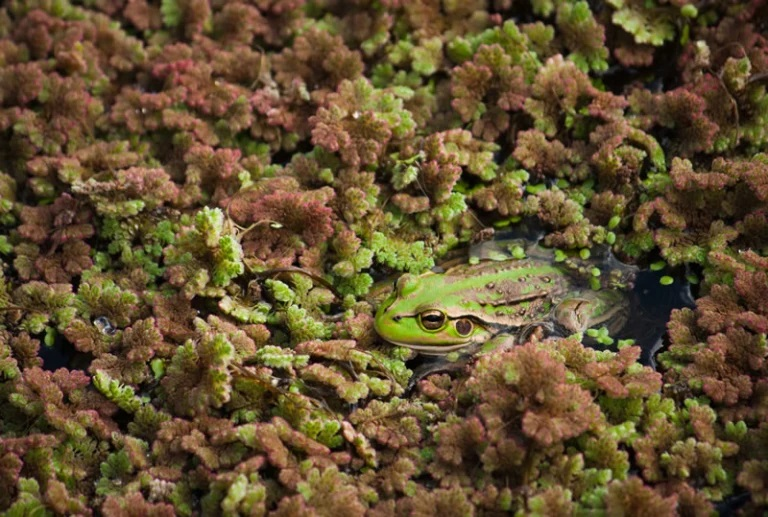
\includegraphics[width=0.9\textwidth]{augmentation/original.jpg}
\caption{Original image}
\end{subfigure}
\begin{subfigure}{0.363\textwidth}
\centering
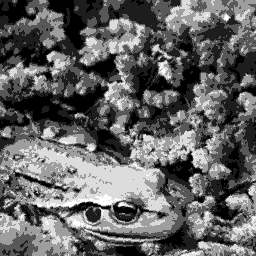
\includegraphics[width=0.9\textwidth]{augmentation/augmented.png}
\caption{Augmented image}
\end{subfigure}

\caption{Example of an image before and after augmentation}
\label{fig:augmentation_example}

\end{figure}

\end{document}